\documentclass[hidelinks,11pt]{article}

\usepackage[english]{babel}

\usepackage{amsmath}
\usepackage{amsfonts}
\usepackage{amssymb}
\usepackage{graphicx}
\usepackage{subcaption}
\usepackage{listings}
\usepackage{caption}
\usepackage{siunitx}
\usepackage{comment}
\usepackage{parskip}
\usepackage{hyperref}
\usepackage{dsfont}
\usepackage{minted}

% separate main text and appendix
\usepackage{selectp}
%\outputonly{1-13}
%\outputonly{14-22}

% preprint
%\usepackage{lineno}
%\usepackage{geometry}
%\geometry{margin=25mm}

%\usepackage{setspace}
%\doublespacing

\usepackage[round]{natbib}
\usepackage{mathtools}
\bibliographystyle{plainnat}

%\captionsetup{
%    font={stretch=2}
%}
% end preprint

\captionsetup{width=0.95\textwidth}

% tolerance for line breaks
\tolerance=400
%\emergencystretch=3em

\title{Simulation and inference on exact solutions of coalescent distributions under diverse demographies.}
\author{Janek Sendrowski\thanks{Bioinformatics Research Center, Aarhus University, Denmark.}, Asger Hobolth\thanks{Department of Mathematics, Aarhus University, Denmark.}\\
Contact:
\href{mailto:sendrowski.janek@birc.au.dk}{\texttt{sendrowski.janek@birc.au.dk}},
    \href{mailto:asger@math.au.dk}{\texttt{asger@math.au.dk}}}

\date{\today}

\begin{document}

    \maketitle

% preprint
%\linenumbers

    \begin{abstract}
        Coalescent theory has proven to be a powerful framework, but exact solutions have so far only been obtainable under relatively simple scenarios, and current simulators such as msprime only provide stochastic solutions, necessitating the use of approximate Bayesian computation (ABC) for parameter inference.
        Recent advancements in phase-type theory now permit exact solutions for all (joint-)moments of coalescent distributions under complex demographic scenarios.
        These include moments of tree height, total branch length and the site-frequency spectrum (SFS) under demographies with multiple demes, varying population sizes and migration rates, multiple merger coalescents, and, to some extent, multiple loci.
        Here we present the theory underlying these developments and propose PhaseGen -- a Python-based software package simulating these moments, and incorporating a maximum likelihood estimation (MLE) framework for parameter inference.
        The package is comprehensively tested, and documented at \href{https://phasegen.readthedocs.io}{\url{phasegen.readthedocs.io}}.
    \end{abstract}


    \section{Introduction}\label{sec:introduction}
    Population genetic simulators are essential tools in evolutionary biology, allowing researchers to explore complex demographic scenarios, develop hypotheses regarding evolutionary processes, and infer parameters under a given demographic model.
    There exists a variety of tools either employing backward or forward simulations, and designed with or without direct parameter inference capabilities.
    Current coalescent-based simulators such as msprime provide stochastic solutions, which gives them great flexibility while mirroring the data generation process~\citep{msprime}. % mention fastsimcoal?
    However, the stochasticity of the results, necessitates the simulation of many replicates for obtaining good estimates of summary statistics, especially when the underlying demographic model is complex and the statistic is based on higher moments.
    Furthermore, parameter inference necessitates the use of approximate Bayesian computation (ABC).

    Another set of tools are forward simulators where the allele frequency trajectories forward in time are described by (often diffusion-based) differential equations~\citep{dadi,moments}.
    The great advantage of forward simulations is that they readily allow for the integration of selection.
    They have, however, different caveats such as model initialization, choice of run times, and they tend to be overall much less efficient that backward simulations. % Too vague? Citation needed
    Furthermore, analytical solutions to the underlying differential equations are rarely available necessitating the use numerical approximations which are not always numerically stable, and higher-order moments are not readily obtainable~\citep{moments}. % more citations, is true?

    Phase-type theory constitutes a unified mathematical framework that offers solutions for mixtures and convolutions of exponential distributions~\citep{phasetype}.
    It is applicable to coalescent theory as the coalescent is phase-type distributed~\citep{phasetype_popgen}.
    One previous limitation of the application of phase-type theory was the restriction to time-homogeneous coalescent processes.
    We describe here how this limit is overcome.  % cite Mogens somehow
    PhaseGen is equipped with a demography interface akin to Msprime, designed to handle temporal changes.
    This is achieved by discretizing the demography into piece-wise constant epochs, enabling the simulation of more intricate demographic scenarios, such as population splits, mergers, and bottlenecks.


    \section{Phase-type distribution}\label{sec:phase-type-distribution}

    \subsection{Introduction}\label{subsec:introduction}

    Consider a Markov jump process $\{X_t\}_{t\geq0}$ with finite state-space $E=\{1, 2, \dots,p\}$ and let $S(t)=\{s(t)_{ij} \}_{i,j=1,\dots,k}$ be the intensity matrix holding the exponential rates of jumping from state $i$ to $j$ at time $t$.
    Define the time until absorption as

% mention that rows sum to zero

    \begin{equation*}
        \tau = \inf\{t >0:X_t \in B\},
    \end{equation*}

    where $B$ is the set of absorbing states. $\tau$ is said to be (time-inhomogeneous) phase-type distributed with state space $E$, initial state vector $\alpha=(\alpha_i)_i$ and intensity matrix $S(t)$, and we write

    \begin{equation*}
        \tau \sim IPH(\alpha,S).
    \end{equation*}

    \subsection{The coalescent}\label{subsec:the-coalescent}
    In the following, we construct a state space for describing the tree height for the standard coalescent.
    For this we require a state space $E=\{1, \dots, n\}$ with $n$ states, where $n$ denotes the number of initial lineages.
    The only absorbing state is $B=\{1\}$ and our transition rates are given by
    \begin{equation*}
        s^d_{ij} = \begin{cases}
                       \binom{i}{2} / N_e & \text{if } i = j - 1, \\ 0 & \text{otherwise,}
        \end{cases}
    \end{equation*}
    where states are indexed with respect to the ordering $\phi(i) = i, i \in E$, and $N_e$ is the effective population size.
    Henceforth, we refer to the state space keeping track of the number of lineages at a time as the default state space.

    In order to obtain more complex summary statistics such as the site-frequency spectrum (SFS), we need to augment the state space to keep track of the number of lineages that subtend $i$ lineages at a time.
    Let each state be an $n$-tuple $e=(a_1, a_2, \dots, a_n)$ with $e_i$ denoting the number of lineages that subtend $i$ lineages.
    Our state space is given by $E=\{e: \sum_i ia_i = n\}$, and the only absorbing state is $B=\{(0, 0, ..., 1)\}$.
    The transition rates are given by~\citep{phasetype_popgen}
    \begin{align*}
        s^b_{\phi(e_1),\phi(e_2)} =
        \begin{cases}
            \binom{a_i}{2} / N_e & \text{if }
            \begin{aligned}[t]
                & e_1=(a_1,\dots,a_n), \\
                & e_2=(a_1,\dots,a_i-2,\dots,a_{2i}+1,\dots,a_{n}), \\
                & a_i \geq 2,
            \end{aligned} \\
            a_i a_j / N_e & \text{if }
            \begin{aligned}[t]
                & e_1=2(a_1,\dots,a_n), \\
                & e_2=(a_1,\dots,a_i-1,\dots,a_j-1,\dots,a_{i+j}+1,\dots,a_{n}), \\
                & a_i a_j \geq 1,
            \end{aligned} \\
            0 & \text{otherwise,}
        \end{cases}
    \end{align*}

    where $\phi$ is an arbitrary ordering.
    We refer to this state space as the block-counting state space, and to $a_i$ as lineage block.
    Details on how to support multiple demes and two loci are shown in the Appendix (\ref{sec:transition_rates}).

    \subsection{Moments}\label{subsec:moments}

    The first moment of $\tau$ can be written as

    \begin{equation*}
        \mathds{E}(\tau) = \int_0^{\infty} \mathds{1}_{E \backslash B}(X_t) dt,
    \end{equation*}

    where $\mathds{1}_{E \backslash B}$ is the indicator function outputting 1 as long as $X_t$ is in a non-absorbing state and 0 otherwise.

    In order to compute more complex summary statistics such as the total branch length and SFS, we want to assign different weights to each state.
    We do this by defining rewards.
    Let $r: E \rightarrow \mathbb{R}_{\geq 0}$ map each state to its chosen reward.

    Then
    \begin{equation*}
        \int_s^{t} r(X_t) dt,
    \end{equation*}

    is the reward accumulated over time $[s, t]$ with respect to $r$.

    In order to compute this quantity, we need to evaluate
    \begin{equation}
        \label{eq:reward_integral}
        \int_s^t P(s,u)R(u)P(s,t) du,
    \end{equation}

    where $P(s,t)$ is a transition matrix describing the probability of transitioning from state $i$ at time $s$ to state $j$ at time $t$, and $R=\{r_{ii}=r(i)\}$ is a (diagonal) reward matrix.

    In practice, determining $P(s,t)$ for time-inhomogeneous processes requires evaluating a product integral, i.e.,

    \begin{equation}
        \label{eq:product_integral}
        P(s,t) = \prod_s^t (I + S(u) du),
    \end{equation}

    which is analytically intractable ($I$ is the identity matrix).
    However, rather than evaluating~\eqref{eq:product_integral} numerically and accept numerically errors, we propose a scheme in which the demography is discretized into $n$ epochs during which $S$ is constant.
    We can then obtain exact solutions under this discretized demography.

    We can use Van Loan's method to evaluate~\eqref{eq:reward_integral} and higher-order moments, including cross moments~\citep{van_loan_popgen,van_loan}.

    Assume for now that $S$ is constant over time.
    Let the Van Loan matrix of order $k$ be the $(k+1) \times (k+1)$ block matrix

    \begin{equation*}
        V_{k}(S, R_1, \dots, R_k) =
        \begin{bmatrix}
            S      & R_1    & 0      & \cdots & 0      & 0      \\
            0      & S      & R_2    & \cdots & 0      & 0      \\
            0      & 0      & S      & \cdots & 0      & 0      \\
            \vdots & \vdots & \vdots & \ddots & \vdots & \vdots \\
            0      & 0      & 0      & \cdots & S      & R_k    \\
            0      & 0      & 0      & \cdots & 0      & S
        \end{bmatrix},
    \end{equation*}

    where $R_i$ are reward matrices.
    Note that we can choose the $R_i$ to be different if we are interested in cross moments.
    Also note that, in practice, we always apply zero rewards to absorbing states.

    Exponentiating $V_k$, we obtain the accumulated reward per state over time $\delta = t - s$:
    \begin{equation*}
        M_k(S, R_1, \dots, R_k,\delta) = \exp(V_k \cdot \delta).
    \end{equation*}

    The reward can be obtained by extracting the upper right block of $M_k$, which we denote $M_k^{sub}$, whence the final moment can be computed as

    \begin{equation*}
        m_k = k! \cdot \alpha \cdot M_k^{sub} \cdot \mathbf{e},
    \end{equation*}

    where $\alpha$ is the initial state vector and $\mathbf{e}$ a vector of ones.

    Now, to obtain the moments for our discretized demography, let $\delta_i$ be the time spent and $S_i$ the intensity matrix in epoch $i$, respectively.
    We can calculate $M_k^i = M_k(S_i, R_1, \dots, R_k,\delta_i)$ for all $i$.
    The matrix containing the total accumulated reward over all epochs is then obtained by

    \begin{equation}
        \label{eq:prod_moments}
        \hat{M}_k = \prod_i{M_k^i}.
    \end{equation}

    In practice, sufficiently many epochs are generated so as to ensure we have reached almost sure absorption.
    Note that~\eqref{eq:prod_moments} constitutes a discretization of the product integral~\eqref{eq:product_integral}.

    The accumulated reward in each state can then be obtained by extracting the upper right block of $\hat{M}_k$, which we denote by $\hat{M}_k^{sub}$.
    The final moment can then be computed as

    \begin{equation*}
        m_k = k! \cdot \alpha \cdot \hat{M}_k^{sub} \cdot e,
    \end{equation*}

    where $\alpha$ is the initial state vector and $e$ a vector of ones.

    To determine the probability of almost sure absorption, we discretize the transition matrix $P_i = \exp(S_i)$, using the same discretization scheme, i.e.,

    \begin{equation*}
        t_{abs} = \min_i\{t: \alpha (\prod_i P_i) e \approx 0 \},
    \end{equation*}

    where $\alpha$ and $e$ are the same as above.

    \subsection{2-epoch example}\label{subsec:2-epoch-example}
    To illustrate the method, assume we have $n=3$ lineages, a single deme, and a 2-epoch demography with $N_e = 1, t \in [0, 2)$ and $N_e = 0.5, t \in [2, \infty)$.
    Assume furthermore we are interested in the variance of the total branch length so that it will suffice to work with the default state space.
    let $(N_1, N_2) = (1, 0.5)$ be the effective population sizes in epochs 1 and 2.
    Also assume we start with 3 lineages in epoch 1 with a probability of 1, so that $\alpha = (1, 0, 0)$.

    We have
    \begin{equation*}
        S_1 = \{s_{ij}\} / N_1 =
        \begin{bmatrix}
            -3 & 3 & 0 \\ 0 & -1 & 1 \\ 0 & 0 & 0
        \end{bmatrix}, \quad
        S_2 = \{s_{ij}\} / N_2 =
        \begin{bmatrix}
            -6 & 6 & 0 \\ 0 & -2 & 2 \\ 0 & 0 & 0
        \end{bmatrix},
    \end{equation*}

    using an ordering of $\phi(i) = 4-i$ where $i$ is the number of lineages, i.e., state 1 is the state with 3 lineages, etc.
    The reward matrix for the total branch length is given by
    \begin{equation*}
        R = \begin{bmatrix}
                3 & 0 & 0 \\ 0 & 2 & 0 \\ 0 & 0 & 0
        \end{bmatrix},
    \end{equation*}

    i.e., we reward each non-absorbing state with its number of lineages.
    The resulting Van Loan matrices are

    \begin{equation*}
        V_1 = \begin{bmatrix}
                  S_1 & R & 0 \\ 0 & S_1 & R \\ 0 & 0 & S_1
        \end{bmatrix} = \left [
            \begin{array}{ccc|ccc|ccc}
                -3 & 3  & 0 & 3  & 0  & 0 & 0  & 0  & 0 \\
                0  & -1 & 1 & 0  & 2  & 0 & 0  & 0  & 0 \\
                0  & 0  & 0 & 0  & 0  & 0 & 0  & 0  & 0 \\
                \hline
                0  & 0  & 0 & -3 & 3  & 0 & 3  & 0  & 0 \\
                0  & 0  & 0 & 0  & -1 & 1 & 0  & 2  & 0 \\
                0  & 0  & 0 & 0  & 0  & 0 & 0  & 0  & 0 \\
                \hline
                0  & 0  & 0 & 0  & 0  & 0 & -3 & 3  & 0 \\
                0  & 0  & 0 & 0  & 0  & 0 & 0  & -1 & 1 \\
                0  & 0  & 0 & 0  & 0  & 0 & 0  & 0  & 0 \\
            \end{array}
            \right ],
    \end{equation*}
    \begin{equation*}
        V_2 = \begin{bmatrix}
                  S_2 & R & 0 \\ 0 & S_2 & R \\ 0 & 0 & S_2
        \end{bmatrix} = \left [
            \begin{array}{ccc|ccc|ccc}
                -6 & 6  & 0 & 3  & 0  & 0 & 0  & 0  & 0 \\
                0  & -2 & 2 & 0  & 2  & 0 & 0  & 0  & 0 \\
                0  & 0  & 0 & 0  & 0  & 0 & 0  & 0  & 0 \\
                \hline
                0  & 0  & 0 & -6 & 6  & 0 & 3  & 0  & 0 \\
                0  & 0  & 0 & 0  & -2 & 2 & 0  & 2  & 0 \\
                0  & 0  & 0 & 0  & 0  & 0 & 0  & 0  & 0 \\
                \hline
                0  & 0  & 0 & 0  & 0  & 0 & -6 & 6  & 0 \\
                0  & 0  & 0 & 0  & 0  & 0 & 0  & -2 & 2 \\
                0  & 0  & 0 & 0  & 0  & 0 & 0  & 0  & 0 \\
            \end{array}
            \right ].
    \end{equation*}

    We then compute the accumulated reward per epoch as
    \begin{equation*}
        % result: [[0.002 0.199 0.798 0.015 0.889 1.69  0.045 2.002 2.316]\n [0.    0.135 0.865 0.    0.541 1.188 0.    1.083 1.293]\n [0.    0.    1.    0.    0.    0.    0.    0.    0.   ]\n [0.    0.    0.    0.002 0.199 0.798 0.015 0.889 1.69 ]\n [0.    0.    0.    0.    0.135 0.865 0.    0.541 1.188]\n [0.    0.    0.    0.    0.    1.    0.    0.    0.   ]\n [0.    0.    0.    0.    0.    0.    0.002 0.199 0.798]\n [0.    0.    0.    0.    0.    0.    0.    0.135 0.865]\n [0.    0.    0.    0.    0.    0.    0.    0.    1.   ]]
        M_1 = \exp(V_1 \cdot \delta_1) \approx
        \left [
            \begin{array}{ccc|ccc|ccc}
                0.002 & 0.199 & 0.798 & 0.015 & 0.889 & 1.69  & 0.045 & 2.002 & 2.316 \\
                0     & 0.135 & 0.865 & 0     & 0.541 & 1.188 & 0     & 1.083 & 1.293 \\
                0     & 0     & 1     & 0     & 0     & 0     & 0     & 0     & 0     \\
                \hline
                0     & 0     & 0     & 0.002 & 0.199 & 0.798 & 0.015 & 0.889 & 1.69  \\
                0     & 0     & 0     & 0     & 0.135 & 0.865 & 0     & 0.541 & 1.188 \\
                0     & 0     & 0     & 0     & 0     & 1     & 0     & 0     & 0     \\
                \hline
                0     & 0     & 0     & 0     & 0     & 0     & 0.002 & 0.199 & 0.798 \\
                0     & 0     & 0     & 0     & 0     & 0     & 0     & 0.135 & 0.865 \\
                0     & 0     & 0     & 0     & 0     & 0     & 0     & 0     & 1
            \end{array}
            \right ],
    \end{equation*}
    \begin{equation*}
        % result [[0.   0.   1.   0.   0.   1.5  0.   0.   1.75]\n [0.   0.   1.   0.   0.   1.   0.   0.   1.  ]\n [0.   0.   1.   0.   0.   0.   0.   0.   0.  ]\n [0.   0.   0.   0.   0.   1.   0.   0.   1.5 ]\n [0.   0.   0.   0.   0.   1.   0.   0.   1.  ]\n [0.   0.   0.   0.   0.   1.   0.   0.   0.  ]\n [0.   0.   0.   0.   0.   0.   0.   0.   1.  ]\n [0.   0.   0.   0.   0.   0.   0.   0.   1.  ]\n [0.   0.   0.   0.   0.   0.   0.   0.   1.  ]]
        M_2 = \exp(V_2 \cdot \delta_2) \approx
        \left [
            \begin{array}{ccc|ccc|ccc}
                0 & 0 & 1 & 0 & 0 & 1.5 & 0 & 0 & 1.75 \\
                0 & 0 & 1 & 0 & 0 & 1   & 0 & 0 & 1    \\
                0 & 0 & 1 & 0 & 0 & 0   & 0 & 0 & 0    \\
                \hline
                0 & 0 & 0 & 0 & 0 & 1   & 0 & 0 & 1.5  \\
                0 & 0 & 0 & 0 & 0 & 1   & 0 & 0 & 1    \\
                0 & 0 & 0 & 0 & 0 & 1   & 0 & 0 & 0    \\
                \hline
                0 & 0 & 0 & 0 & 0 & 0   & 0 & 0 & 1    \\
                0 & 0 & 0 & 0 & 0 & 0   & 0 & 0 & 1    \\
                0 & 0 & 0 & 0 & 0 & 0   & 0 & 0 & 1
            \end{array}
            \right ].
    \end{equation*}

    where $\delta_1 = 2$ and $\delta_2 = t_{abs} \coloneqq 31$, the time until almost sure absorption.

    To obtain the total accumulated reward over all epochs, we compute
    \begin{equation}
        \label{eq:prod_moments_example}
        % result: [[0.    0.    1.    0.    0.    2.797 0.    0.    5.477]\n [0.    0.    1.    0.    0.    1.865 0.    0.    3.053]\n [0.    0.    1.    0.    0.    0.    0.    0.    0.   ]\n [0.    0.    0.    0.    0.    1.    0.    0.    2.797]\n [0.    0.    0.    0.    0.    1.    0.    0.    1.865]\n [0.    0.    0.    0.    0.    1.    0.    0.    0.   ]\n [0.    0.    0.    0.    0.    0.    0.    0.    1.   ]\n [0.    0.    0.    0.    0.    0.    0.    0.    1.   ]\n [0.    0.    0.    0.    0.    0.    0.    0.    1.   ]]
        \hat{M} = M_2 \cdot M_1 \approx
        \left [
            \begin{array}{ccc|ccc|ccc}
                0 & 0 & 1 & 0 & 0 & 2.797 & 0 & 0 & 5.477 \\
                0 & 0 & 1 & 0 & 0 & 1.865 & 0 & 0 & 3.053 \\
                0 & 0 & 1 & 0 & 0 & 0     & 0 & 0 & 0     \\
                \hline
                0 & 0 & 0 & 0 & 0 & 1     & 0 & 0 & 2.797 \\
                0 & 0 & 0 & 0 & 0 & 1     & 0 & 0 & 1.865 \\
                0 & 0 & 0 & 0 & 0 & 1     & 0 & 0 & 0     \\
                \hline
                0 & 0 & 0 & 0 & 0 & 0     & 0 & 0 & 1     \\
                0 & 0 & 0 & 0 & 0 & 0     & 0 & 0 & 1     \\
                0 & 0 & 0 & 0 & 0 & 0     & 0 & 0 & 1
            \end{array}
            \right ],
    \end{equation}

    from which we can extract the total accumulated reward in the upper right block. We have

    \begin{equation*}
        % result: [[0.    0.    5.477]\n [0.    0.    3.053]\n [0.    0.    0.   ]]
        \hat{M}^{sub} \approx \left [
            \begin{array}{ccc}
                0 & 0 & 5.477 \\
                0 & 0 & 3.053 \\
                0 & 0 & 0
            \end{array}
            \right ].
    \end{equation*}

    We can then compute the (uncentered) second moment by
    \begin{equation*}
        m_2 \approx 2! \cdot \alpha \cdot \hat{M}^{sub}\cdot e = 2 \left [
            \begin{array}{ccc}
                1 & 0 & 0
            \end{array}
            \right ] \left [
            \begin{array}{ccc}
                0 & 0 & 5.477 \\
                0 & 0 & 3.053 \\
                0 & 0 & 0
            \end{array}
            \right ] \left [
            \begin{array}{c}
                1 \\ 1 \\ 1
            \end{array}
            \right ] \approx 10.955.
    \end{equation*}

    After obtain the mean $m_1$, using the same method, we can obtain the variance by

    \begin{equation*}
        \sigma^2 = m_2 - m_1^2 \approx 10.955 - 2.797^2 \approx 3.132.
    \end{equation*}


    \section{Runtime}\label{sec:runtime}

    Let $n$ be the number of lineages, $k$ the moment's order, and $d$ the number of demes.
    Furthermore, let $P_0(n, k)$ be the number of partitions of $n$ into $k$ non-negative integer parts. % let $P(n)$ be the number of integer partitions of $n$ and

    % TODO add number of loci here
    The Van Loan matrix for the default state space has size
    \begin{equation*}
        \text{order}(V^k(S^d)) = (k + 1) \cdot \sum_{i=1}^{n} P_0(i, d),
    \end{equation*}
    and for the block-counting state space, we have
    \begin{equation*}
        \text{order}(V^k(S^d)) = (k + 1) \cdot \sum_{i=1}^{n} \prod_{j \in P_n} P_0(j, d),
    \end{equation*}

    where $P_n$ is the set of partitions of $n$ (cf.\ Figure~\ref{fig:state_space_sizes} for examples).

    % mention time complexity of matrix exponentiation, state space construction, and demography discretization
    % also mention growth rate of state space size with respect to n, k, d
    % Talk about precision of Padé approximation


    \section{Code examples}\label{sec:code-examples}

    In the code snippet below, we define a coalescent distribution with a 2-deme, 4-epoch demography and a total number of lineages of \texttt{n=8}.
    As our ancestry model we choose the beta coalescent with \texttt{alpha=1.7}.
    Upon construction the different distributions are available.

    \begin{minted}{python}
import phasegen as pg

coal = pg.Coalescent(
    n=pg.LineageConfig({'pop_0': 3, 'pop_1': 5}),
    model=pg.BetaCoalescent(alpha=1.7),
    demography=pg.Demography(
        pop_sizes={
            'pop_1': {0: 1.2, 5: 0.1, 5.5: 0.8},
            'pop_0': {0: 1.0}
        },
        migration_rates={
            ('pop_0', 'pop_1'): {0: 0.2, 3: 0.3},
            ('pop_1', 'pop_0'): {0: 0.5}
        }
    )
)

    \end{minted}

    We now proceed to plotting some quantities, namely the demography, tree height distribution, expected SFS and correlation matrix of different SFS bins.
    Note that we adjust the maximum time shown to be the 99th percentile of the tree height distribution.
    The output of the snippet below is shown in Figure~\ref{fig:simple-example}

    \begin{minted}{python}
import numpy as np
import matplotlib.pyplot as plt

_, axs = plt.subplots(2, 2, figsize=(9, 7))
t = np.linspace(0, coal.tree_height.quantile(0.99), 100)

coal.demography.plot(ax=axs[0, 0], show=False, t=t)
coal.tree_height.plot_pdf(ax=axs[0, 1], show=False)
coal.sfs.mean.plot(ax=axs[1, 0], show=False, title='SFS')
coal.sfs.corr.plot(ax=axs[1, 1], show=False, title='2-SFS')

plt.tight_layout()
plt.show()
    \end{minted}

    \begin{figure}[H]
        \centering
        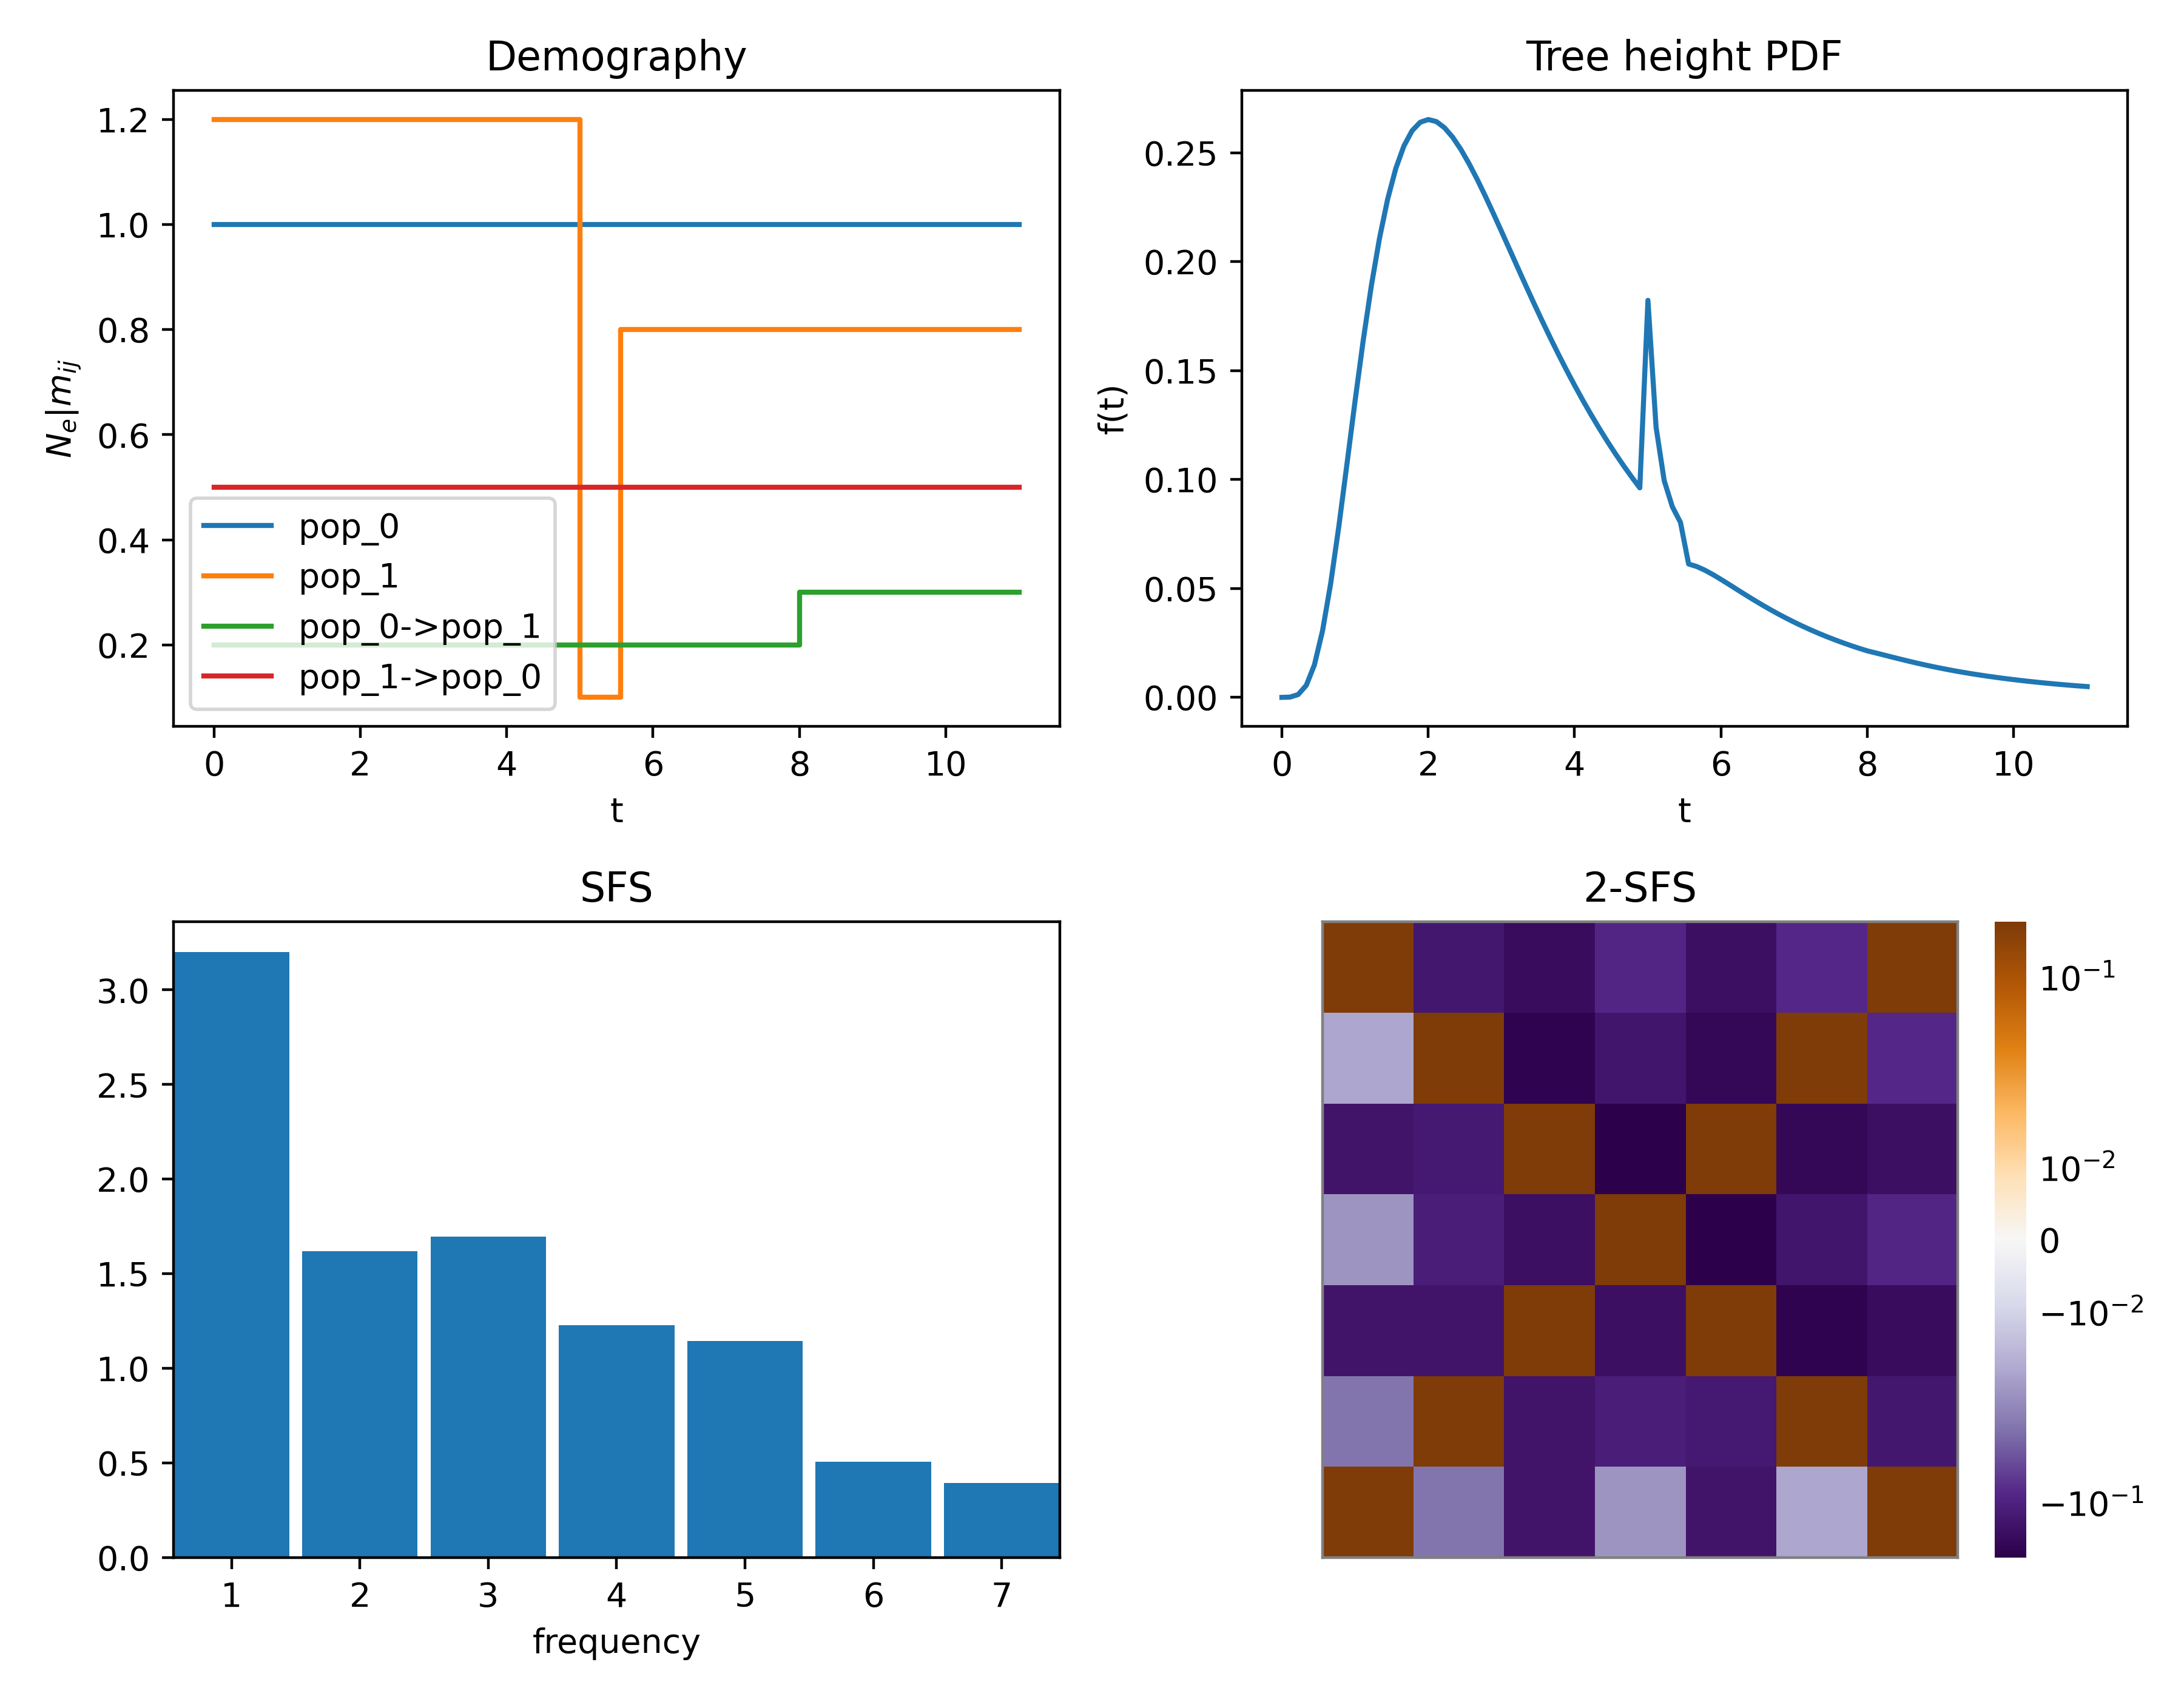
\includegraphics[width=\textwidth]{figures/manuscript_example}
        \caption{
            Output from code snippet in Section \ref{sec:code-examples}.
            \textbf{Top left}: population sizes and migration rates over time.
            \textbf{Top right}: tree height distribution. \textbf{Bottom left}: expected SFS.
            \textbf{Bottom right}: 2-SFS correlation matrix.
        }
        \label{fig:simple-example}
    \end{figure}

    \subsection{MLE Inference}\label{subsec:mle-inference}

    \subsection{More complex moments}\label{subsec:other-quantities}


    \section{Discussion}\label{sec:discussion}

    \section*{Acknowledgements}

    \newpage
    \bibliography{refs}

    \newpage
    \appendix
    \nolinenumbers

\renewcommand{\thefigure}{\thesection.\arabic{figure}}
\renewcommand{\thetable}{\thesection.\arabic{table}}


\section{Transition Rates}\label{sec:transition_rates}

\subsection{Migration}\label{subsec:migration}

\subsubsection{Default State Space}\label{subsubsec:migration_default}
Let each state be described by $\mathbf{e}=(d_1, \ldots, d_m)$, where $d_i$ is the number of lineages in deme $i$, and $m$ is the number of demes.
Migration events are not allowed to occur concurrently with coalescence or recombination events, and only one lineage can migrate at a time.
We have
\begin{align*}
    s^d_{\phi(\mathbf{e}_1),\phi(\mathbf{e}_2)} =
    \begin{cases}
        m_{ij} \cdot n_i & \text{if }
        \begin{aligned}[t]
            & \mathbf{e}_1=(a_1,\dots,a_n), \\
            & \mathbf{e}_2=(a_1,\dots,a_i-1,\dots,a_j+1,\dots,a_{n}), \\
            & a_i \geq 1,
        \end{aligned} \\
        0 & \text{otherwise,}
    \end{cases}
\end{align*}
where $m_{ij}$ is the migration rate from deme $i$ to deme $j$ backwards in time, and $n_i$ is the number of lineages in deme $i$ prior to the migration event.

\subsubsection{Block-counting State Space}\label{subsubsec:migration_block_counting}
Let each state be described by $e=(\mathbf{d}_1, \ldots, \mathbf{d}_m)$, where $\mathbf{d}_i=(a_{i1}, \ldots, a_{in})$ are the lineage block counts in deme $i$, and $n$ is the initial number of lineages.
We have
\begin{align*}
    s^b_{\phi(\mathbf{e}_1),\phi(\mathbf{e}_2)} =
    \begin{cases}
        m_{ij} \cdot n_{ij} & \text{if }
        \begin{aligned}[t]
            & \mathbf{e}_1=(\mathbf{d}_1,\dots,\mathbf{d}_n), \\
            & \begin{aligned}[t]
                  \mathbf{e}_2 &= ( \\
                  & \mathbf{d}_1, \dots, \\
                  & (a_{i1},\dots,a_{ik}-1,\dots,a_{in}), \dots, \\
                  & (a_{j1},\dots,a_{jl}+1,\dots,a_{jn}), \dots, \\
                  & \mathbf{d}_n \\
            \end{aligned} \\
            & ), \\
            & a_{ik} \geq 1,
        \end{aligned} \\
        0 & \text{otherwise,}
    \end{cases}
\end{align*}
where $n_{ij}$ is the number of lineages in block $j$ of deme $i$ prior to the migration event.
We have one absorbing state for each deme in which the final coalescence event can take place.
When modeling more than one locus, we additionally need to make sure that migration events on modify the lineage block counts consistently across linked loci.

\begin{figure}[H]
    \centering
    \includegraphics[width=\textwidth]{figures/migration_two_lineages_default}
    \caption{
        Transition rates for migration in a two-deme model with two lineages using the default state space.
        Each note represents a state, and each edge a transition.
        States are described by a 2-tuple which respresent the number of lineages and linked lineages, respectively.
        All migration rates and population sizes are 1.
        Green nodes indicate the initial states, and red nodes the absorbing states.
    }
    \label{fig:migration_two_lineages_default}
\end{figure}

%Each state is parameterized by a 3-dimensional array $e_{ijk}$.
%For $i = 0$, $j$ is the deme index and $k$ is the lineage block index of the number of lineages in each deme and lineage block.
%For $i = 1$, $j$ is the deme index and $k$ is the lineage block index of the number of linked lineages in each deme and lineage block.
%For the default state space, there is only one lineage block holding all lineages.
%In alternative terminology, the two elements along the first dimension of $\mathbf{e}$ correspond to the number of lineages and linked lineages, respectively.
%The second dimension to the demes and the third dimension to lineage blocks.
%For example, $[[[1] [1]], [[0] [0]]]$ indicates that there is one lineage in each deme and no linked lineages.

\subsection{Beta Coalescent}\label{subsec:beta-coalescent}

\subsubsection{Default State Space}\label{subsubsec:beta_coalescent_default}
Let $E=\{1,2,\ldots,n\}$, where each state describes the number of present lineages, and $n$ is the initial number of lineages.
Let $\alpha \in (1, 2)$.
Then the probability of $k$ out of $b$ lineages coalescing is given by~\citep{beta_coalescent}
\begin{align*}
    \lambda_{b,k} = B(k - \alpha, b - k + \alpha) / B(\alpha, 2 - \alpha).
\end{align*}

The transition rates are given by
\begin{align*}
    s^d_{e_1,e_2} =
    \begin{cases}
        \binom{b}{k} \lambda_{b,k} / N_e & \text{if }
        \begin{aligned}[t]
            & \mathbf{e}_1=b, \\
            & \mathbf{e}_2=b - k + 1, \\
            & b \geq k,
        \end{aligned} \\
        0 & \text{otherwise.}
    \end{cases}
\end{align*}
Note that a different generation time scaling other than $N_e$ is also implemented in PhaseGen.

\subsubsection{Block-counting State Space}\label{subsubsec:beta_coalescent_block_counting}

\subsection{Dirac Coalescent}\label{subsec:dirac-coalescent}

\subsubsection{Default State Space}\label{subsubsec:dirac_coalescent_default}

\subsubsection{Block-counting State Space}\label{subsubsec:dirac_coalescent_block_counting}

\subsection{Recombination}\label{subsec:recombination}
\subsubsection{Default State Space}\label{subsubsec:recombination_default}

\begin{figure}[H]
    \centering
    \includegraphics[width=\textwidth]{figures/recombination_two_lineages}
    \caption{
        Transition rates for 2-locus recombination model with two lineages using the default state space.
        % TODO explain state space parametrization
        States are described by a 2-tuple which respresent the number of lineages and linked lineages, respectively.
    }
    \label{fig:recombination_two_lineages}
\end{figure}

\subsubsection{Block-counting State Space}\label{subsubsec:recombination_block_counting}


\section{State Space Size}\label{sec:state_space}

\begin{figure}[H]
    \centering
    \includegraphics[width=\textwidth]{figures/state_space_size}
    \caption{
        State space size for different numbers of lineages and demes.
        The different subplots consider the default state space with one locus and two loci, as well as the block-counting state space with one locus.
    }
    \label{fig:state_space_sizes}
\end{figure}


\section{Runtime}\label{sec:runtime-appendix}

\begin{figure}[H]
    \centering
    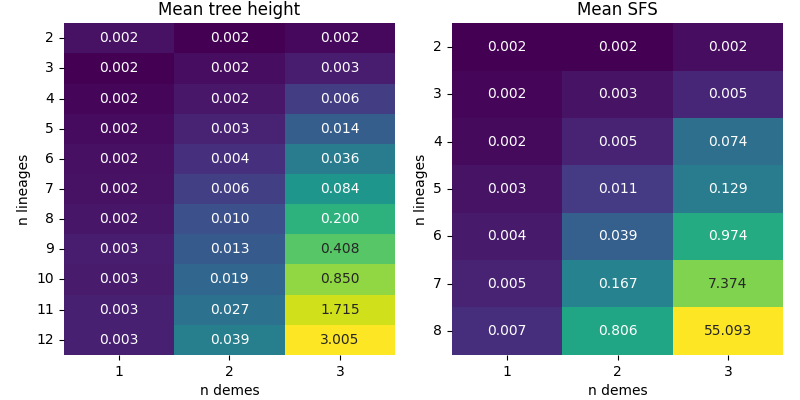
\includegraphics[width=\textwidth]{figures/executions_times}
    \caption{
        Total execution times in seconds for different numbers of lineages and demes.
        The different subplots consider the default and block-counting state spaces with one locus.
        Note that the computation of the SFS required $n$ independent matrix exponentiations, where $n$ is the number of lineages.
    }
    \label{fig:executions_times}
\end{figure}



\end{document}
